\chapter{函数与极限}
\section{利用定义证明极限}
\subsection{自变量趋于有限值时函数的极限}
\tdefination[函数极限1]
设函数$f(x)$在点$x_0$的某一去心邻域\index{QXLY@去心领域}\footnote{去心邻域指的是以$x_0$为中心的连续区间$U(x_0)$去掉中心$x_0$后的新区间,记为$U\degree (x_0 )$.特别注意的是,去心邻域仅在中心$x_0$处没有定义,其它点都有定义.}内有定义.如果存在常数$A$,对于任意给定的正数$\varepsilon$(不论它多么小),总存在正数$\delta$使得当$x$满足不等式$0<|x-x_0 |<\delta$时,对应的函数值$f(x)$都满足不等式
\begin{equation}
|f(x)-A|<\varepsilon
\end{equation}
那么常数$A$就叫做函数$f(x)$当$x \to x_0$的\dy[极限]{JX},记作
\begin{equation}
\lim\limits_{x\to x_0}f(x)=A \huo f(x)\to A(x \to x_0)
\end{equation}
\sj \sj 
\begin{figure}[!htb]
	\begin{center}
		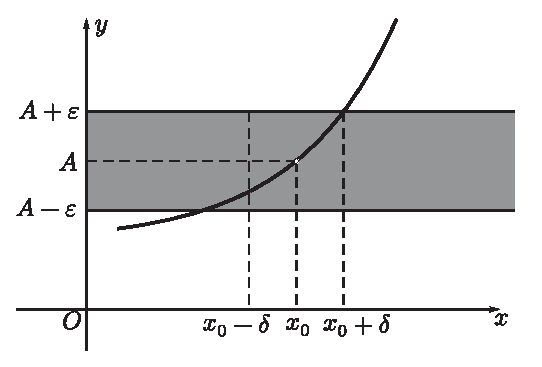
\includegraphics[scale=0.8]{pictures/C-1/极限1.eps}
	\end{center}
	\sj \sj 
	\caption{极限的定义图解}
\end{figure}
\sj
\subsection{自变量趋于无穷大时函数的极限}
\tdefination[函数极限2]
设函数$f(x)$在当$|x|$大于某一正数时恒有定义.如果存在常数$A$,对于任意给定的正数$\varepsilon$(不论它多么小),总存在正数$X$使得当$x$满足不等式$|x|>X$时,对应的函数值$f(x)$都满足不等式
\begin{equation}
|f(x)-A|<\varepsilon
\end{equation}
那么常数$A$就叫做函数$f(x)$当$x \to x_0$的\dy[极限]{JX},记作
\begin{equation}
\lim\limits_{x\to \infty}f(x)=A \huo f(x)\to A(x \to \infty )
\end{equation}

\subsection{无穷小与无穷大}
\tdefination[无穷小]
如果函数$f(x)$当$x\to x_0\left(\mbox{或}x \to \infty  \right) $时的极限为$0$,那么称函数$f(x)$为当$x\to x_0\left(\mbox{或}x \to \infty  \right) $时的\dy[无穷小]{WQX}.记为
\begin{equation}
\lim\limits_{x \to x_0}f(x)=0,\lim\limits_{x\to \infty}f(x)=0.
\end{equation}
特别地,以$0$为极限的数列${x_n}$称为$n\to \infty$时的\dy[无穷小]{WQX}.
\jg

\defination[无穷大]
设函数$f(x)$在$x_0$的某一去心邻域内有定义(或$|x|$趋于某一正数时有定义).如果对于任意给定的正数$M$(不论它多么大),总存在正数$\delta$(或正数$X$),只要$x$适合不等式$0<|x-x_0|<\delta$(或$|x|>X$),对应函数值$f(x)$总满足不等式
\begin{equation*}
|f(x)|>M
\end{equation*}
那么称函数$f(x)$为当$x\to x_0\left(\mbox{或}x \to \infty  \right) $时的\dy[无穷大]{WQD}.记为
\begin{equation}
\lim\limits_{x \to x_0}f(x)=\infty,\lim\limits_{x\to \infty}f(x)=\infty.
\end{equation}

\subsection{单侧极限}
\tdefination[左极限]
在 $\lim\limits_{x \to x_0}f(x)=A$的定义中,把$0<|x-x_0 |<\delta$改为$x_0-\delta <x<x_0$ ,那么$A$就叫做函数$f(x)$当$x \to x_0$时的\dy[左极限]{ZJX}.记作
\begin{equation}
\lim\limits_{x \to x_0^-}f(x)=A \huo f(x_0^-)=A \huo \lim\limits_{x \to x_0 - 0}f(x)=A
\end{equation}

\defination[右极限]
在 $\lim\limits_{x \to x_0}f(x)=A$的定义中,把$0<|x-x_0 |<\delta$改为$x_0 <x<x_0+\delta$ ,那么$A$就叫做函数$f(x)$当$x \to x_0$时的\dy[右极限]{YJX}.记作
\begin{equation}
\lim\limits_{x \to x_0^+}f(x)=A \huo f(x_0^+)=A \huo \lim\limits_{x \to x_0 + 0}f(x)=A
\end{equation}

\subsection{利用定义求函数的极限的解题方法}
\texample[可以直接求得$\delta$与$\varepsilon$的关系]
任意一个$\varepsilon$满足$|f(x)-A|<\varepsilon$,都能找到一个正数$\delta$使$0 < |x - x_0| < \delta$或$|x| > \delta$ ,这就说明了$\varepsilon$与$\delta $有个对应关系,即
\begin{equation}
\delta=\varphi(\varepsilon)
\end{equation}
\par $\delta=\varphi(\varepsilon)$这个关于$\varepsilon$的函数可以是任意的.所以我们利用极限的定义来证明某个函数的极限时,只需找到$\varepsilon$和$\delta$之间的对应关系.这时,我们可以先利用$|f(x)-A|<\varepsilon$这个条件,然后构造出 $|x - x_0| < \varphi(\varepsilon)$的形式即可.(对于求数列的极限时$\delta$换成$N$即可.)

\examples 证明下列极限\\[0.5em]
\hspace*{0.8em} $1.\,\,\lim\limits_{x \to 3}2x-1=5$

\proof  设$\exists \delta,\forall \varepsilon$,当$0<|x-3|<\delta $时,$|2x-1-5|=|2x-6|=2|x-3|<\varepsilon$\quad \quad 【构造$|x-x_0 | < \varphi (\varepsilon)$】\\[0.5em]
即$\displaystyle |x-3|<\frac{\varepsilon}{2}$,故取$\displaystyle \delta = \frac{\varepsilon}{2}$时成立,证毕.\\[1.5em]
\hspace*{0.8em} $2.\,\,\displaystyle \lim\limits_{x \to \infty }\frac{1}{x}=0$\\[1em]
\proof  设$\exists N,\forall \varepsilon$,当$|x|>N$时,$\displaystyle \left| \frac{1}{x}-0\right| =\left| \frac{1}{x}\right|<\varepsilon$\hspace{13em}【构造$|x-x_0 | < \varphi (\varepsilon)$】\\[0.5em]
即$\displaystyle |x|>\frac{1}{\varepsilon}$,故取$\displaystyle N = \frac{1}{\varepsilon}$时成立,证毕.\\

\example[不能直接求得$\delta$与$\varepsilon$的关系]
\noindent 【方法一】放缩法\vspace{0.8em}
\par 这个时候我们可以将$|f (x) - A|$进行适当的放大,使得$\delta $与$\varepsilon$的关系容易求得,一般的放缩方法有:\\[0.5em]
\noindent (1)  将分母恒大于零的部分(可以含$x$)删去;\\[0.5em]
\noindent (2)  将分子恒小于零的部分删去(可以含$x$);\\[0.5em]
\noindent (3)  将幂函数的底数部分进行放缩.

\examples 证明$\displaystyle \lim\limits_{x \to 1}\sqrt{3x+1}=2.$

\proof 设$\exists \delta,\forall \varepsilon$,当$0<|x-1|<\delta $时,$\displaystyle |\sqrt{3x+1}-2|=\frac{3(x-1)}{\sqrt{3x+1}+2}\le \frac{3}{2}|x-1|<\varepsilon$\hspace{4em}【放缩构造】\\[0.5em]
即$\displaystyle |x-1|<\frac{2}{3}\varepsilon$,又$\displaystyle \sqrt{3x+1}$定义域为$\displaystyle x>-\frac{1}{3}$,那么$\displaystyle x-1>-\frac{4}{3}$,在一定范围内有$\displaystyle |x-1|<\frac{4}{3}$\hspace{1em}【判断定义域】\\[0.5em]
故取$\displaystyle \delta = \min \left\lbrace  \frac{2}{3}\varepsilon,\frac{4}{3} \right\rbrace $时成立,证毕.\hspace{27em}【取最小值】\\

\noindent 【方法二】先设后求再取值法\vspace{0.8em}
\par 放缩不是唯一的方法,我们还可以先设后求再取$\delta $最小值.\\[0.5em]
\noindent (1)  先化简式子,且含$|x-a|$项,这个时候可以用该方法;\\[0.5em]
\noindent (2)  设$\delta $的值为$f(a)$ (可以含$a,x$,也可以是常数);\\[0.5em]
\noindent (3)  解出$x$的范围,对非$|x - a|$的项进行放缩,将式子放大,同时使得非$|x - a|$的项转换为常量;\\[0.5em]
\noindent (4)  反解出$\delta = \varphi (\varepsilon)$;\\[0.5em]
\noindent (5)  取$\delta = \min \lbrace f(a),\varphi(\varepsilon)\rbrace$.\vspace{0.5em}
\par 当然通常放缩法和先设后求再取值法会结合用,这样就可以解决大部分题目.\vspace{0.5em}
\par 但是在后面的证明过程中,一般简单的函数极限可以直接用,所以一般情况下不会用定义证明极限.

\examples 证明$\lim\limits_{x \to a}x^2=a^2$

\proof 由于$|x^2-a^2|=|(x-a)(x+a)|=|x-a|\cdot |x+a| $,\hspace{15em}【找到$|x-a|$项】\\[0.5em]
设$\displaystyle |x-a|<\frac{1}{2}$,则$\displaystyle |x+a|=|x-a+2a|\le |x-a|+|2a|<\frac{1}{2}+|2a|.$【赋值$|x-a|$项,并放缩得出未知项的范围】\\[0.5em]
所以,设$\exists \delta,\forall \varepsilon$,当$0<|x-1|<\delta $时,$\displaystyle |x^2-a^2|=|x-a|\cdot |x+a|<\left( \frac{1}{2}+|2a|\right)|x-a|<\varepsilon $,\\[0.5em]
即$\displaystyle|x-a|<\frac{\varepsilon}{\frac{1}{2}+2|a|}$.\hspace{28em}【反解出$|x-a|$的范围】\\[0.5em]
故取$\displaystyle \delta = \min \left\lbrace  \frac{\varepsilon}{\frac{1}{2}+2|a|},\frac{1}{2} \right\rbrace $时成立,证毕.\hspace{24.5em}【取最小值】\\

\subsection{证明函数的极限不存在的方法}
\ttheorem[序列极限]
设函数$f (x)$在$a$点的一个空心邻域内有定义,并且$\lim\limits_{x \to a}f(x)=l$.假若是一串在该空心邻域内取值的序列,且
\begin{equation*}
\lim\limits_{n \to \infty}x_n=a
\end{equation*}
则有
\begin{equation}
\lim\limits_{n \to \infty}f(x_n)=l
\end{equation}
\par 这个定理为我们提供了一种\textbf{证明函数极限不存在的办法}:对于一个定义在$a$点的某空心邻域内的函数$f(x)$,如果能找到两串序列$\lbrace x'_n \rbrace $与$\lbrace x''_n\rbrace$它们都在$a$的该空心邻域内取值,且当$n\to \infty $时都以$a$为极限,而极限$\lim\limits_{n \to \infty }x'_n$与 $\lim\limits_{n \to \infty }x''_n$都存在但不相等,则$f(x)$在$x \to a$时不可能有极限.\jg

\example[证明函数的极限不存在]
\sj \examples 证明:函数$\displaystyle \sin \frac{1}{x}$在$x\to 0$时没有极限.

\proof 取$\displaystyle x'_n=\frac{1}{2n\pi }$,则$\displaystyle \sin \frac{1}{x'_n}=0$;而取$\displaystyle x''_n=\frac{1}{2n\pi+\frac{\pi}{2} }$,则$\displaystyle \sin \frac{1}{x'_n}=1.$\\[0.5em]
这时由于$n \to \infty \Rightarrow x'_n\to 0,x''_n \to 0, $且
\begin{equation*}
\lim\limits_{n \to \infty} \sin \frac{1}{x'_n} \ne \lim\limits_{n \to \infty} \sin \frac{1}{x''_n} 
\end{equation*}
因此,函数$\displaystyle \sin \frac{1}{x}$在$x\to 0$时没有极限.

\section{利用极限运算法则和两个准则求极限}
\subsection{极限运算法则}
\ttheorem[极限运算法则1]
两个无穷小的和是无穷小.

\tl 有限个无穷小的和是无穷小.
\newpage
\theorem[极限运算法则2]
有界函数与无穷小的乘积是无穷小.

\tl 常数与无穷小的乘积是无穷小.

\tl 有限个无穷小的乘积是无穷小.\jg

\theorem[极限运算法则3]
如果$\lim f(x) = A, \lim g(x) = B$(这些函数都必须存在极限),那么
\begin{equation}
\lim [f(x)\pm g(x)]=\lim f(x)\pm \lim g(x)=A \pm B
\end{equation}
\begin{equation}
\lim[f(x)\cdot g(x)]=\lim f(x)\cdot \lim g(x)=A\cdot B
\end{equation}
若$B\ne 0$,那么
\begin{equation}
\lim \left[ \frac{f(x)}{g(x)}\right] =\frac{\lim f(x)}{\lim g(x)}=\frac{A}{B}
\end{equation}

\tl 如果$\lim f(x)$存在,而$c$为常数,那么
\begin{equation}
\lim [cf(x)]=c \lim f(x)
\end{equation}

\tl 如果$\lim f(x)$存在而$n$为正整数,那么
\begin{equation}
\lim [f(x)]^n=[\lim f(x)]^n
\end{equation}

\theorem[极限运算法则4]
如果$\varphi(x) \ge \psi(x),$而$\lim \varphi(x)=A,\lim \psi(x)=B,$则$A \ge B.$\jg

\subsection{极限运算准则}
\ttheorem[单调有界数列极限一定存在]
(1)  \quad 若$x_{n+1} \le x_n(n\mbox{为正整数})$,且$x_n \ge m,$则$\lim\limits_{n \to \infty }x_n = A $存在,且$A \ge m$;\jg
\par (2)  \quad 若$x_{n+1} \ge x_n(n\mbox{为正整数})$,且$x_n \le M,$则$\lim\limits_{n \to \infty }x_n = A $存在,且$A \le M$.

\theorem[夹逼定理]
设$g(x) \le f(x) \le h(x)$,若$\lim\limits_{x \to m}g(x)=A,\lim\limits_{x \to m}=A,(-\infty \le m \le +\infty)$则$\lim\limits_{x \to m}f(x)=A.$\jg

\subsection{例题}
\texample[利用极限运算法则和两个准则求极限]\sj
\examples 证明:$\lim\limits_{n \to \infty}q^n=0.(|q|<1)$

\proof 设$\displaystyle |q|=\frac{1}{1+a},a>0,$则$\displaystyle 0< q^n=\frac{1}{(1+a)^n}=\frac{1}{C^0_na^0=C^1_na^1+C^2_na^2+\cdots+C^n_na^n}<\frac{1}{C^1_na^1}=\frac{1}{na}.$\\[0.5em]
又$\displaystyle \lim\limits_{n \to \infty}\frac{1}{na}=0,\lim\limits_{n\to \infty}0=0,$由夹逼定理可得
\begin{equation*}
\lim\limits_{n\to \infty}0 \le \lim\limits_{n \to \infty}q^n \le \lim\limits_{n \to \infty}\frac{1}{na}
\end{equation*}
故$\lim\limits_{n \to \infty}q^n=0.$\jg

\examples 证明:$\displaystyle a_n=\frac{a^n}{n!}(a\mbox{是大于1的任意常数})$存在极限.

\proof 当$n>[a]+1$时,有
\begin{equation*}
0\le a_n =\frac{a^{[a]}}{[a]!}\cdot \frac{a}{[a]+1}\cdot \frac{a}{[a]+2}\cdot \,\,\cdots \,\,\cdot \frac{a}{n}<\frac{a^{[a]}}{[a]!}\cdot \frac{a}{n}
\end{equation*}
注意到$\displaystyle \frac{a^{[a]}}{[a]!}$是一个常数,所以$\displaystyle \lim\limits_{n \to \infty}\frac{a^{[a]}}{[a]!}\cdot \frac{a}{n}=0,$由夹逼定理可得
\begin{equation*}
\lim\limits_{n \to \infty}a_n=0.
\end{equation*}

\examples 设常数$a>1,$对于任意自然数$k$,证明:
\begin{equation*}
\lim\limits_{n \to \infty}\frac{n^k}{a^n}=0.
\end{equation*}
\hspace*{-0.5em}\proof 令$t=a-1$,则$t>0$,那么
\[
a_n=(1+t)^n=1+nt+\frac{n(n-1)}{2!}t^2+\cdots+\frac{n(n-1)\cdot(n-k)}{(k+1)!}t^{k+1}+\cdots+t^n,
\]
因此,当$n>1$时,$\displaystyle a^n>\frac{n(n-1)\cdots(n-k)}{(k+1)!}t^{k+1}$,于是
\[
0 \le \frac{n^k}{a^n}\le \frac{n^k}{\displaystyle \frac{n(n-1)\cdots(n-k)}{(k+1)!}t^{k+1}}=\frac{(k+1)!}{t^{k+1}}\cdot \frac{n^k}{n(n-1)\cdots(n-k)}=\frac{(k+1)!}{t^{k+1}}\cdot\frac{n^k}{\lambda_{k+1}n^{k+1}+\lambda_kn^k+\cdots+\lambda_1n+\lambda_0}
\]
其中$\lambda_0,\lambda_1,\cdots,\lambda_{k+1}$均为非零常数.注意到$\displaystyle \frac{(k+1)!}{t^{k+1}}$为常数,则
\begin{equation*}
\begin{split}
&\quad \, \lim\limits_{n \to \infty}\frac{(k+1)!}{t^{k+1}}\cdot\frac{n^k}{\lambda_{k+1}n^{k+1}+\lambda_kn^k+\cdots+\lambda_1n+\lambda_0}\\
&=\lim\limits_{n \to \infty}\frac{(k+1)!}{t^{k+1}}\cdot\frac{1}{n}\cdot \frac{n^k}{\lambda_{k+1}+\lambda_kn^{-1}+\cdots+\lambda_1n^{-k}+\lambda_0n^{-k-1}}=0
\end{split}
\end{equation*}
因此,由夹逼定理可得
\begin{equation*}
\lim\limits_{n \to \infty}\frac{n^k}{a^n}=0.
\end{equation*}

\section{利用等价无穷小求极限}
\subsection{无穷小的分类}
\tdefination[无穷小的分类]
设$\alpha,\beta $是同一变化过程中的无穷小,$\displaystyle \lim \frac{\beta}{\alpha}$是这一过程的极限,$c$为常数,那么\\[0.5em]
\noindent (1) \quad $\displaystyle \lim \frac{\beta }{\alpha}=0$,则称$\beta $是$\alpha $的\dy[高阶无穷小]{GJWQX},记作$\beta = o(\alpha)$.\\[0.5em]
\noindent (2) \quad  $\displaystyle \lim \frac{\beta }{\alpha}=\infty$,则称$\beta $是$\alpha $的\dy[低阶无穷小]{DJWQX1}.\\[0.5em]
\noindent (3) \quad  $\displaystyle \lim \frac{\beta }{\alpha}=c \ne 0$,则称$\beta $是$\alpha $的\dy[同阶无穷小]{TJWQX}.\\[0.5em]
\noindent (4) \quad  $\displaystyle \lim \frac{\beta }{\alpha}=1$,则称$\beta $是$\alpha $的\dy[等价无穷小]{DJWQX2},记作$\beta \sim \alpha$.\\[0.5em]
\noindent (3) \quad  $\displaystyle \lim \frac{\beta }{\alpha^k}=c \ne 0$,则称$\beta $是$\alpha $的\dy[$k$阶无穷小]{KJWQX}.\\[0.5em]
\color{black}{{\CJKfamily{heiti}注意}}\quad 0与``0"的区别\\[0.5em]
\noindent (i)\quad ``0"指的是无穷小,设$\alpha$是某一变化过程中的无穷小,也就是说$x$趋于某一值时,极限为0.\\[0.5em]
\noindent (ii)\quad 当0指的是实数0时,$\lim 0 \cdot f(x)=0$,这与$f(x)$无关,即使$\lim f(x)=\infty$,其结果仍然是0,因为0在这里时实数,而不是无穷小.\jg

\subsection{常见的等价无穷小}
\ttheorem[常见的等价无穷小]
以下等价无穷小均为$x \to 0$这一变化过程,其中$x$也可替换为一个函数,即$f(x) \to 0$的情况也适用.
\begin{equation}
\tan x \sim \sin x \sim x \sim \arcsin x \sim \arctan x
\end{equation}
\begin{equation}
\ln (1+x) \sim x
\end{equation}
\begin{equation}
x \sim \e^x -1
\end{equation}
\begin{equation}
1-\cos x \sim \frac{x^2}{2}
\end{equation}
\begin{equation}
\sec x -1 =\frac{1}{\cos x}-1 \sim \frac{x^2}{2}
\end{equation}
\begin{equation}
(1+x)^a-1 \sim 1-ax
\end{equation}
\begin{equation}
a^x-1 \sim \ln a \cdot x \,(a>0,a \ne 1)
\end{equation}
\subsection{等价无穷小求极限的本质}
等价无穷小求极限本质上是极限与1的相乘,而有等价无穷小的定义,1可以换成极限$\displaystyle 1=\lim\limits_{x \to x_0}\frac{\alpha }{\beta}$,再运用极限乘法运算法则计算即可.

\example[等价无穷小的误用]\sj
\examples \label{例 1.8}求极限$\displaystyle \lim\limits_{x \to 0}\frac{\tan x -\sin x}{\sin^3 x}$.

\errsolve  由于$\tan \sim \sin x \sim x$得$\displaystyle \lim\limits_{x \to 0}\frac{\tan x -\sin x}{\sin^3 x}=\lim\limits_{x \to 0}\frac{x-x}{\sin^3 x}=\lim\limits_{x \to 0}0=0.$

\errreason  在运用等价无穷小的时候没有考虑极限运算法则成立的条件.

\solvereason $\displaystyle \lim\limits_{x \to 0}\frac{\tan x -\sin x}{\sin^3 x}=\lim\limits_{x \to 0}\frac{\tan x}{\sin^3 x} - \lim\limits_{x \to 0}\frac{\sin x}{\sin^3 x}$实际上运用了法则$\lim [f(x)-g(x)]=\lim f(x)-\lim g(x),$\\[1em]即完整的错解解题步骤应为
\begin{equation*}
\lim\limits_{x \to 0}\frac{\tan x -\sin x}{\sin^3 x}=\lim\limits_{x \to 0}\frac{\tan x}{\sin^3 x} - \lim\limits_{x \to 0}\frac{\sin x}{\sin^3 x}
=\lim\limits_{x \to 0}\frac{\tan x}{\sin^3 x}\cdot \lim\limits_{x \to 0} \frac{x}{\tan x}-\lim\limits_{x \to 0}\frac{x}{\sin^3 x}
\end{equation*}
而极限运算法则成立的条件是$\lim f(x),\lim g(x)$存在,而$\displaystyle \lim\limits_{x \to 0}\frac{\tan x}{\sin^3 x}$不存在,因此解题错误.

\solve $\displaystyle \lim\limits_{x \to 0}\frac{\tan x -\sin x}{\sin^3 x}=\lim\limits_{x \to 0}\frac{\sin x(\sec x-1)}{\sin^3 x}=\lim\limits_{x \to 0}\frac{\sec x-1}{\sin^2 x} \cdot \lim\limits_{x \to 0}\frac{\frac{x^2}{2}}{\sec x -1} \cdot \lim\limits_{x \to 0}\frac{\sin x^2}{x^2}
=\frac{\frac{x^2}{2}}{x^2}=\frac{1}{2}.$\jg

\examples 求极限$\displaystyle \lim_{x \to 0} \frac{\sin \left(x^2 \sin{\frac{1}{x}}\right) }{x}.$

\errsolve $\displaystyle \lim_{x \to 0}\frac{\sin \left(x^2 \sin{\frac{1}{x}}\right) }{x}=\lim_{x \to 0}\frac{x^2 \sin \frac{1}{x}}{x}=\lim_{x \to 0}x\sin\frac{1}{x}=0.$

\errreason 对极限概念的理解不清晰,不仔细,没有严格判断等价无穷小的定义式是否满足极限的定义.

\solvereason 实际上,该错误解答的完整版本应该为:
\[
\lim_{x \to 0} \frac{\sin \left(x^2 \sin{\frac{1}{x}}\right) }{x}=\lim_{x \to 0} \frac{\sin \left(x^2 \sin{\frac{1}{x}}\right) }{x}\cdot\frac{x^2\sin \frac{1}{x}}{\sin \left( x^2 \sin \frac{1}{x}\right) }=\lim_{x \to 0}\frac{x^2\sin\frac{1}{x}}{x}=\lim_{x \to 0}x\sin \frac{1}{x}=0.
\]
但是极限
\[
\lim_{x \to 0}\frac{x^2\sin \frac{1}{x}}{\sin \left( x^2\sin \frac{1}{x}\right) }
\]
中,若$\displaystyle \sin \frac{1}{x}$取0,则这个极限式无意义(分母为0).故$\displaystyle x \ne \frac{1}{k \pi}(k \in Z).$\hspace*{11.5em}【判断定义域】\\[0.5em]
\hspace*{2em}这样的话,在点$x = 0$的任何一个去心邻域中都有无穷多个点没有定义,所以不存在一个去心邻域满足该极限式,
故极限不存在.\hspace*{24em}【判断是否能找到满足的去心邻域】\\[0.5em]
这里再次强调一下0与``0"的区别: 分母为0的时候并不是指无穷小量,而是真正意义上的0.

\solve 设$\exists \delta, \forall \varepsilon,$使得当$|x-0|<\delta$时,$\displaystyle \left| \frac{\sin \left( x^2\sin\frac{1}{x}\right) }{x}-0\right|<\varepsilon$,\\[0.5em]
由不等式$|\sin x|\le |x|$,得
\[
\left| \frac{\sin \left( x^2\sin\frac{1}{x}\right) }{x}\right| \le \left| \frac{ \left( x^2\sin\frac{1}{x}\right) }{x}\right| =\left| x \sin \frac{1}{x} \right|.
\]
由$\displaystyle \left| \sin \frac{1}{x} \right| \le 1$,得
\[
\left| \frac{\sin \left( x^2\sin\frac{1}{x}\right) }{x}\right| \le \left| \frac{ \left( x^2\sin\frac{1}{x}\right) }{x}\right| =\left| x \sin \frac{1}{x} \right|.\le |x|<\varepsilon
\]

\subsection{例题}
\sj
\example[等价无穷小的运用]\sj
在下面的例题中,为了方便,省略了含有等价无穷小本质的式子.但是建议读者在实际做题的过程中还是要写完整,方便利用定义检查式子的合理性.

\examples 求极限$\displaystyle \lim_{x \to \infty}\left(\cos \frac{3}{x} \right)^{x^2} $

\solve 令$\displaystyle t=\frac{1}{x}$,则$x=\frac{1}{t},x\to \infty ,t \to 0.$
\[
\lim_{x \to \infty}\left(\cos \frac{3}{x} \right)^{x^2} =\lim_{t \to 0}(\cos 3t)^{\frac{1}{t^2}}=\lim_{t \to 0}\left[\left( 1-2\sin^2\frac{3t}{2}\right)^{\frac{1}{2\sin^2\frac{3t}{2}}} \right]^{\frac{2\sin^2\frac{3t}{2}}{t^2}} =\e^{\displaystyle -\lim_{t \to 0}\frac{2\sin^2\frac{3t}{2}}{t^2}}
\]
因为$\displaystyle \lim_{t \to 0}\frac{2\left( \displaystyle \frac{3t}{2}\right)^2 }{t^2}=\frac{9}{2},\,\therefore \lim_{x \to \infty }\left(\cos \frac{3}{x} \right)^{x^2}=\e^{ \displaystyle  -\lim_{t \to 0}\frac{2\sin^2\frac{3t}{2}}{t^2}}=\e ^{-\frac{9}{2}} $

\solveother 令$\displaystyle t=\frac{1}{x}$,则$\displaystyle x=\frac{1}{t},x\to \infty ,t \to 0.$
\[
\lim_{x \to \infty}\left( \cos \frac{3}{x}\right)^{x^2} =\lim_{t \to 0}(\cos 3t)^{\frac{1}{t^2}}=\e^{\lim\limits_{t \to 0}\ln(\cos 3t)^{\frac{1}{t^2}}}
\]
\[
\because \lim\limits_{t \to 0}\frac{1}{t^2}\ln(\cos 3t)=\lim\limits_{t \to 0}\frac{1}{t^2}\ln (\cos 3t)=\lim\limits_{t \to 0}\frac{1}{t^2}\ln \left[1+\left(-2\sin^2\frac{3t}{2}\right)\right]=\lim_{t \to 0}\frac{-2\sin^2\frac{3t}{2}}{t^2}=\lim\limits_{t \to 0}\frac{-2\left(\frac{3t}{2}\right)^2}{t^2}=-\frac{9}{2}.
\]
\[
\therefore \lim_{x \to \infty}\left( \cos \frac{3}{x}\right)^{x^2}=\lim\limits_{t \to 0}(\cos 3t)^{\frac{1}{t^2}}=\e^{\lim\limits_{t \to 0}\ln(\cos 3t)^{\frac{1}{t^2}}}=\e^{-\frac{9}{2}}.
\]

\inference[等价无穷小类型\uppercase\expandafter{\romannumeral1}]
以上是利用两种等价无穷小的解法,下面对这两种等价无穷小的用法归类.(这两个极限选一个用即可).若一个极限表达式有下列的形式(或者经过换元、取对数等方法变成这种形式),则很有可能用到这两种极限.
\begin{equation}
\lim f(x)^{g(x)}
\end{equation}
其中$\lim f(x)=1,\lim g(x)$存在.

解法一\qquad 变形为:
\begin{equation}
	\lim\big[1+\big(f(x)-1\big)\big]^{g(x)}=\lim\big[1+\big(f(x)-1\big)\big]^{\frac{g(x)[f(x)-1]}{f(x)-1}}=\e^{\lim g(x)\cdot [f(x)-1]}
\end{equation}
而此时$\lim g(x) \cdot [f(x)-1]$是容易求得的.


解法二\qquad 变形为:
\begin{equation}
\lim\big[1+\big(f(x)-1\big)\big]^{g(x)}=\e^{\lim \ln[1+\left( f(x)-1\right) ]}=\e^{\lim g(x)\cdot [f(x)-1]}
\end{equation}
而此时$\lim g(x) \cdot [f(x)-1]$也是容易求得的.

\examples 已知函数$f(x)$满足$\displaystyle \lim_{x \to 0}\frac{\sqrt{1+f(x)\sin 2x}-1}{\e^{3x}-1}=2$,求$\displaystyle \lim_{x \to 0}f(x).$

\solve $\displaystyle \lim_{x \to 0}\frac{\sqrt{1+f(x)\sin 2x}-1}{\e^{3x}-1}=\lim\limits_{x \to 0}\frac{1/2f(x)\sin 2x}{3x}=\lim_{x \to 0}\frac{1/2f(x)2x}{3x}=\frac{1}{3}\lim_{x\to 0}f(x)=2.$
\[
\therefore \lim_{x \to 0}f(x)=6.
\]

下面给出一个较难看出错误的例题.

\examples \label{例 1.12}求极限$\displaystyle \lim_{x \to 0}\left[ \frac{(1+x)^{\frac{1}{x}}}{\e}\right]^{\frac{1}{x}}.$

\errsolve $\displaystyle \lim_{x \to 0}\left[ \frac{(1+x)^{\frac{1}{x}}}{\e}\right]^{\frac{1}{x}}=\lim_{x \to 0}\left[ \frac{\e}{\e}\right]^{\frac{1}{x}}=1.$

\errreason 在运用等价无穷小的时候没有考虑极限运算法则成立的条件.

\solvereason $\displaystyle \lim_{x \to 0}\left[ \frac{(1+x)^{\frac{1}{x}}}{\e}\right]^{\frac{1}{x}}=\e^{\lim\limits_{x \to 0}\frac{1}{x}\ln\frac{(1+x)^{\frac{1}{x}}}{\e}},$
\[
\lim_{x \to 0}\frac{1}{x}\ln\frac{(1+x)^{\frac{1}{x}}}{\e}=\lim\limits_{x \to 0}\frac{1}{x}\left[ \ln(1+x)^{\frac{1}{x}} -\ln \e\right]=\lim\limits_{x \to 0}\frac{1}{x}\cdot\lim\limits_{x \to 0}\left[ \ln(1+x)^{\frac{1}{x}} -\ln \e\right]=\lim_{x \to 0}\frac{1}{x} \cdot \lim\limits_{x \to 0} \left[ \ln \e -\ln \e \right]=0.
\]
实际上,在$\displaystyle \lim\limits_{x \to 0}\frac{1}{x}\left[ \ln(1+x)^{\frac{1}{x}}-\ln \e \right]=\lim\limits_{x \to 0}\frac{1}{x}\cdot\lim\limits_{x \to 0}\left[ \ln(1+x)^{\frac{1}{x}} -\ln \e\right]$中用到了$\lim \big[f(x)\cdot g(x)\big]=\lim f(x) \cdot \lim  g(x)$,即用到了极限运算法则,而$\displaystyle \lim_{x \to 0}\frac{1}{x}$不存在,因此这种运算错误.

\solve $\displaystyle \lim_{x \to 0}\left[ \frac{(1+x)^{\frac{1}{x}}}{\e}\right]^{\frac{1}{x}}=\lim_{x \to 0}\left\lbrace1+\left[\frac{(1+x)^{\frac{1}{x}}}{\e}-1\right]\right\rbrace^{\frac 1x}=\lim_{x \to 0}\left\lbrace1+\left[\frac{(1+x)^{\frac{1}{x}}}{\e}-1\right]\right\rbrace^{ \frac{1}{(1+x)^{\frac 1x}-1}\cdot \frac{(1+x)^{\frac 1x}-1}{x}},$
\[
\because \lim\limits_{x \to 0}\left[\frac{(1+x)^{\frac{1}{x}}}{\e}-1\right]=0,\therefore \lim_{x \to 0}\left\lbrace1+\left[\frac{(1+x)^{\frac{1}{x}}}{\e}-1\right]\right\rbrace^{ \frac{1}{(1+x)^{\frac 1x}-1}\cdot \frac{(1+x)^{\frac 1x}-1}{x}}=\e^{\lim\limits_{x\to 0}\frac{(1+x)^\frac 1x-1}{x}},
\]
\[
\because \lim\limits_{x\to 0}\frac{\frac{(1+x)^\frac 1x}{\e}-1}{x}=\lim\limits_{x\to 0}\frac{(1+x)^\frac 1x-\e}{\e x}=\lim\limits_{x \to 0}\frac{\e^{\frac{1}{x}\ln(1+x)}-\e}{\e x}\xlongequal[]{\e^x-1 \sim x} \lim\limits_{x \to 0}\frac{\frac{1}{x}\ln(1+x)-1}{x}=\lim_{x \to 0}\frac{\ln (1+x)-x}{x^2}
\]
\[
\xlongequal[]{\ln(1+x)-x\sim-\frac{1}{2}x^2} \lim\limits_{x \to 0}\frac{-\frac{1}{2}x^2}{x^2}=-\frac{1}{2}
\]
\[
\therefore \lim_{x \to 0}\left[ \frac{(1+x)^{\frac{1}{x}}}{\e}\right]^{\frac{1}{x}}=\e^{\lim\limits_{x\to 0}\frac{(1+x)^\frac 1x-1}{x}}=\e^{-\frac{1}{2}}=\frac{\sqrt{\e}}{\e}.
\]

\inference[等价无穷小求极限]\sj
\begin{enumerate}
	\item 判断并构造等价无穷小的类型(7 种);
	\item 利用等价无穷小求极限的本质列出计算式;
	\item 判断等价无穷小的极限式中能否找到满足定义域的去心邻域使得极限存在:
	\begin{enumerate}[(i)]
		\item 若存在,则利用等价无穷小解题;
		\item 若不存在,则用其它方法求解(如利用函数定义、夹逼准则等).
	\end{enumerate}
	\item 检验计算的每一步是否都符合极限运算法则的前提条件.
\end{enumerate}

\warn[
	\hspace*{2em}1. 以上等价无穷小都只在$x\to 0$的情况下才成立,$x$趋于其它值时不成立.\\
	\hspace*{2em}2. 只有等价无穷小的定义式存在极限的前提下,即在函数$f (x)$的定义域内能找到一个完整的去心邻域,$x$才可以用任意函数$f(x)$替换.若等价无穷小的定义式都不存在极限,又谈何等价无穷小.\\
	下面给出常见的一些不可以用等价无穷小替换的函数.\jg\\
	\examples $\displaystyle x \to 0,\sin\left(x \sin \frac 1x\right) \not \sim x\sin \frac{1}{x},\sin\left(x\cos \frac 1x\right)\not \sim x \cos \frac 1x$\\
	\hspace*{2em}3. 在运用等价无穷小计算极限的时候要特别要注意在替换的过程中只有符合极限的运算法则,才可以进行
替换(通常极限的运算法则不明显,需要仔细计算),前面已经给出了两个详细的例子.
]

\section{函数连续性}
\subsection{函数连续性的定义}
\tdefination[函数在某点的连续性\uppercase\expandafter{\romannumeral1}]
设函数$y=f(x)$在点$x_0$的某一邻域内有定义,如果
\begin{equation}
\lim\limits_{\Delta x \to 0}\Delta y=\lim\limits_{\Delta x \to 0}\big[f(x_0+\Delta x)-f(x_0)\big]=0.
\end{equation}
那么就称函数$y=f(x)$在点$x_0$处\dy[连续]{LX}.

\defination[函数在某点的连续性\uppercase\expandafter{\romannumeral2}]
设函数$y=f(x)$在点$x_0$的某一邻域内有定义,如果
\begin{equation}
\lim\limits_{x \to x_0} f(x)=f(x_0).
\end{equation}
那么就称函数$y=f(x)$在点$x_0$处\dy[连续]{LX}.\jg

即$f(x)$在点$x_0$处连续$\Longleftrightarrow \forall \varepsilon>0,\exists \delta>0,$当$|x-x_0|<\delta$时,都有$|f(x)-f(x_0)|<\varepsilon$

\defination[左连续]
如果$\lim\limits_{x \to x_0^-}f(x)=f(x_0^-)$存在且等于$f(x_0)$,即$f(x_0^-)=f(x_0)$,那么就称函数$y=f(x)$在点$x_0$处\dy[左连续]{ZLX}.

\defination[右连续]
如果$\lim\limits_{x \to x_0^+}f(x)=f(x_0^+)$存在且等于$f(x_0)$,即$f(x_0^+)=f(x_0)$,那么就称函数$y=f(x)$在点$x_0$处\dy[右连续]{YLX}.

\warn[\hspace*{2em}函数在某点连续的充要条件是在该点的左极限和右极限都存在且都等于函数该点处的函数值.或者说函数在该点既左连续又右连续.(证明函数在某点处是否连续的方法)]

\defination[函数在某个区间的连续性]
在区间上每一点都连续的函数,叫做在该区间上的连续函数,或者说函数在该区间上连续.如果区间包括端点,那么函数在右端点是指右端点的左连续,在左端点是指左端点的右连续.

\blackbf[连续函数的图形是一条连续而不间断的线(可能是直线,也可能是曲线).]
\jg

\subsection{函数的间断点}
\tdefination[函数的间断点]
设函数$y=f(x)$在点$x_0$的某一邻域内有定义.在此前提条件下,如果函数有下列三种情况之一:\\[0.5em]
(1) 在$x=x_0$处没有定义;\hspace{12em}(2) 虽在$x=x_0$处有定义,但是$\displaystyle \lim\limits_{x \to x_0}f(x)$不存在;\\[0.5em]
(3) 虽在$x=x_0$处有定义,$\displaystyle \lim\limits_{x \to x_0}f(x)$存在,但$\displaystyle \lim_{x \to x_0}f(x) \ne f(x_0)$.\\[0.5em]
那么就称函数$f(x)$在点$x_0$处不连续,而点$x_0$称为函数$f(x)$的\dy[不连续点]{BLXD}或\dy[间断点]{JDD}.

如果$x_0$是函数$f(x)$的间断点,但左极限$f(x_0^-)$和右极限$f(x_0^+)$都存在,那么点$x_0$就称为函数$f(x)$的\dy[第一类间断点]{DYLJDD},不是第一类间断点的任何间断点都是\dy[第二类间断点]{DELJDD}.常见的具体分类见下表\ref{函数间断点的分类}.
\begin{table}[!htb]
	\centering
	\renewcommand{\arraystretch}{1}
	\setlength{\tabcolsep}{16mm}{
		\begin{tabular}{cc}
			\toprule[1.5pt] 
			\rowcolor[gray]{0.9} \blackbf[第一类间断点] & \blackbf[第二类间断点] \\
			\midrule
			可去间断点 & 无穷间断点\\
			\midrule
			 跳跃间断点 & 震荡间断点\\
			\bottomrule[1.5pt]
		\end{tabular}  
	}
	\caption{函数间断点的分类}
	\renewcommand{\arraystretch}{1}
	\label{函数间断点的分类}
\end{table} 

\defination[无穷间断点]
若$x_0$是函数$f(x)$的间断点,且$\lim\limits_{x \to x_0}f(x)=\infty $,那么我们称点$x_0$是函数的\dy[无穷间断点]{WQJDD}.\jg

\simpleexamples $\displaystyle x=\frac{\pi}{2}$是函数$y=\tan x$的无穷间断点.

\defination[振荡间断点]
若$x_0$是函数$f(x)$的间断点,且当$x \to x_0$时,函数值在多个值之间变动无穷多次,那么我们称点$x_0$是函数$f(x)$的\dy[振荡间断点]{ZDJDD}.\jg

\simpleexamples $\displaystyle x = 0$是函数$\displaystyle y =\sin\frac{1}{x}$的振荡间断点.

\warn[
\kg 若点$x_0$是函数$f(x)$的振荡间断点,那么在函数$f(x)$在点$x_0$处的任意的去心邻域都无确定的值.
进一步说,如果函数$f(x)$的导函数是$f'(x)$,点$x_0$是导函数$f'(x)$的振荡间断点,那么在$x_0$的任意去心邻域中函数$f(x)$的导数都不存在.
]

\defination[可去间断点]
若点$x_0$是函数$f(x)$的间断点,且$f(x)$在点$x_0$处没有定义,而$\lim\limits_{x \to x_0}f(x)=f(x_0),$那么我们称点$x_0$是函数$f(x)$的\dy[可去间断点]{KQJDD}.\jg

\simpleexamples $\displaystyle x=1$是函数$\displaystyle y=\frac{x^2-1}{x-1}$的可去间断点.

\defination[跳跃间断点]
若点$x_0$是函数$f(x)$的间断点,且$f(x)$在点$x_0$处有定义,而$f(x_0^-)=f(x_0^+)$,那么我们称点$x_0$是函数$f(x)$的\dy[跳跃间断点]{TYJDD}.

\simpleexamples $\displaystyle x=0$是函数
$
\displaystyle
\begin{cases}
x-1,x<0\\
0\,\,\,\,\,\,\,\,\,\,\,,x=0\\
x+1,x>0
\end{cases}
$
的跳跃间断点.



